\documentclass{article}
\usepackage{amsmath}
\usepackage{hyperref}
\usepackage{graphicx}
%\usepackage{darkmode}
%\enabledarkmode
\title{Aquatic Problem Set}
\author{David Hunt}
\date{\today}

\begin{document}

\maketitle

\section*{Theory Problems}
\subsection*{Problem 1}
\subsection*{Problem Statement}
Suppose you run two OLS regression models on disjoint datasets, one of $Y_1$ (Mx1) onto $X_1$ (Mx1) and the other 
of $Y_2$ (Nx1) onto $X_2$ (Nx1). Both models come without intercept. Let the resulting coefficients be $\beta_1$ and $\beta_2$ respectively. 
Suppose now you co-fit another OLS model on the union of two datasets also without intercept. 
You therefore have a linear regression of Y ((M+N)x1) onto X ((M+N)x1), where Y is a concatenation of $Y_1$ and $Y_2$ and X is a concatenation of $X_1$ and $X_2$. 

\subsection*{Assumptions I'm making about the datasets}
\begin{itemize}
    \item \textbf{Linearity}: size of $X_1$ is close to  size $X_2$.
    \item \textbf{No Intercepts}: Interceps are centered at zero.
\end{itemize}

\subsection*{Part A}
\textbf{Question}: a.	Given $\beta_1$ and $\beta_2$, what is the possible range of the coefficient $\beta$ if you run the OLS regression of Y onto X?
\newline
\subsection*{Answer and Explanation}
The possible range of the coefficient $\beta$ is $min(\beta_1,\beta_2) <= \beta <= max(\beta_1,\beta_2)$.\newline 
Define:\newline  
$$Y_1 = B_1 + X_1\beta_1 + \epsilon_1$$
$$Y_2 = B_2 + X_2\beta_2 + \epsilon_2$$
OLS estimates of $\beta_1$ and $\beta_2$ are: 
$$ \beta_1 = \frac{X_1 ^\top Y_1}{X_1 ^\top X_1}$$
$$ \beta_2 = \frac{X_2 ^\top Y_2}{X_2 ^\top X_2}$$
The combined Y and X are: 
$$Y = \begin{bmatrix} Y_1 \\ Y_2 \end{bmatrix}$$
$$X = \begin{bmatrix} X_1 \\ X_2 \end{bmatrix}$$
OLS Estimate for the combined datasets are:\footnote[1]{OLS \url{https://en.wikipedia.org/wiki/Ordinary_least_squares}}
$$ \beta = \frac{X ^\top Y}{X ^\top X}$$
Inputting that into the formula yields:
$$ \beta = \frac{\begin{bmatrix} X_1 \\ X_2 \end{bmatrix} ^\top \begin{bmatrix} Y_1 \\ Y_2 \end{bmatrix}}{\begin{bmatrix} X_1 \\ X_2 \end{bmatrix} ^\top \begin{bmatrix} X_1 \\ X_2 \end{bmatrix}}$$
Breaking down the matrix multiplication yields:
$$ \beta = \frac{X_1 ^\top Y_1 + X_2 ^\top Y_2}{X_1 ^\top X_1 + X_2 ^\top X_2}$$
Substituting the OLS estimates of $\beta_1$ and $\beta_2$ into the equation yields:
$$ \beta = \frac{X_1 ^\top Y_1 + X_2 ^\top Y_2}{X_1 ^\top X_1 + X_2 ^\top X_2} = \frac{X_1 ^\top (X_1\beta_1 + \epsilon_1) + X_2 ^\top (X_2\beta_2 + \epsilon_2)}{X_1 ^\top X_1 + X_2 ^\top X_2}$$
Showing that the range of $\beta$ is a weighted average of the two coefficients.

$$min(\beta_1,\beta_2) <= \beta <= max(\beta_1,\beta_2)$$

\subsection*{Part B}
\textbf{Question}: b. weekhat if instead all three regressions of $Y_1$ on $X_1$, of $Y_2$ on $X_2$ and of $Y$ on $X$ are run with intercept? 
Let $\beta_1$, $\beta_2$ and $\beta$ be the corresponding parameters associated with $X_1$, $X_2$ and $X$. 
Given $\beta_1$ and $\beta_2$, what is the possible range of $\beta$? You may assume the answer is an interval without gaps.

\subsection*{Answer and Explanation}

\subsection*{interesting edgecases}
\begin{itemize}
    \item If the coefficents are exactly opposite then the resultant beta will be 0. i.e. -1 and 1 will yield 1 
    \item if the size of one data set is grossly larger than the other, the resultant beta will be closer to the larger dataset.
    \item If the size of the datasets are the same, the resultant beta will be the average of the two coefficients.
\end{itemize}
If we run with an intercept vs without the resultant coefficent $\beta$ will be the same as without the intercept. 

defining the coefficent of an OLS regression as: 
$$\beta = \frac{X ^\top Y}{X ^\top X}$$ or 
$$\beta = \frac{\sum_{i-1}^n{}(X-\hat{X})(Y - \hat{Y})}{\sum_{i=1}{n}(X-\hat{X})^2} $$
then the combination of the OLS betas from $X_1$ and $X_2$ will be:
$$\beta = \frac{\sum_{i-1}^n{}(X_1-\hat{X_1})(Y_1 - \hat{Y_1}) + \sum_{i-1}^n{}(X_2-\hat{X_2})(Y_2 - \hat{Y_2})
                }{\sum_{i=1}{n}(X_1-\hat{X_1})^2 + \sum_{i=1}{n}(X_2-\hat{X_2})^2
                } ==> \beta_1 + \beta_2 $$
yielding: 
$$min(\beta_1,\beta_2) <= \beta <= max(\beta_1,\beta_2)$$

\subsection*{Part C}
\textbf{Question}: Again, assume no intercepts are fitted in any of the three regressions as in part a. Further assume that all $(x, y)$ pairs in $(X, Y)$ are drawn i.i.d. from a zero-mean 2D multivariate Gaussian distribution.
                     Given $\beta_1$ and $\beta_2$, what's your best guess at $\beta$? You may take reasonable approximations in your solution.

\subsection*{Answer and Explanation}
Given that the data is drawn from a zero-mean 2D multivariate Gaussian distribution, the best guess at $\beta$ is the same as $beta_1$ and $beta_2$.

Since the mean of a gaussain distribution is zero and covariance is\footnote[2]{Pulled some formulas from here \url{https://cs229.stanford.edu/section/gaussians.pdf} and \url{https://en.wikipedia.org/wiki/Multivariate_normal_distribution}}:
$$\Sigma = \begin{bmatrix} \sigma_{x}^2 & \rho\sigma_x\sigma_y\\ \rho\sigma_x\sigma_y & \sigma_{y}^2 \end{bmatrix}$$

$$ \beta_1 = \frac{Cov(X,Y)}{Var(X,Y)} = \rho \frac{\sigma_y}{\sigma_x}$$
Meaning that the variacnes are equal and don't impact the coefficient.

thus in expectancy the best guess at $\beta$ is the same as $\beta_1$ and $\beta_2$. 
As we're drawing from the same i.i.d dataset the resultant beta will be the same as the individual betas.


\subsection*{Problem 2}
\subsection*{Problem Statement}
Suppose that you have two matrices of regressors X1 and X2 where X1 is Nxk and X2 is N*(f-k). 
You fit a multiple regression model for a target variable Y onto X1 obtaining residuals e and a QR decomposition of the matrix X1. 
\subsection*{Part A}
\textbf{Question}: You want to find which one of the additional variables contained in X2 will reduce the residual sum of squares the most when included with the ones from X1. Detail an efficient procedure to obtain this. 
In my opinion the easiset way do evaluate this is to do a form of grid search on the additional varabiles to reduce the RSS here. 

There is a slighly intelligent way that we could do this to avoid having to search through the whole dataset which would occurn in $O(n^2)$ time.
First we could perform some separate regressions to identifiy the correlations between variables as variables that are already in the dataset and highly correlated are unlikely to help us reduce variance any further. 
After that we could perform a regression on the dataset and then add the variables one by one to see if they reduce the RSS evaluating them in order of least correlation to the original dataset, (this looks a lot like PCA). 

\subsection*{Part B}

This bleeds in from part A, but once we have identified the most promissing set of varabiles to include from $X_2$ we can then grid search through them to identify the best combination of variables, 
downside of doing this is this occurs in $O(2^n)$ time as our dimensionaly blows out with the addition of variables.
However there are some techniques that we could use to reduce the number of variables that we need to search through as this looks more like an operations research problem.
some helpfull techniques include 
\begin{itemize}
    \item Regularization of the regression model \footnote[3]{wiki \url{https://en.wikipedia.org/wiki/Regularization_(mathematics)}}
    \item Parrellelization of the search through the dataset
    \item Dimensionality reduction techniques such as PCA \footnote[4]{wiki \url{https://en.wikipedia.org/wiki/Principal_component_analysis}}
\end{itemize}

I'm sure there's a more mathematically optimal solution to this problem but these ways will get you there and reduce the search time to \textit{nearly} optimal.

\subsection*{Data Exercise}
Please see the attached \textit{.ipynb} file for the code implementation of the problem set. \newline
A poetry.toml file is included to install the necessary dependencies to run the code.

\subsection*{Part 1}
Please find the attached graph on exploratory data analysis of the dataset.
The dataset does not apepar to be time series data, but rather a collection of numerical data.
In addition, there were a few outliers in the model that I winsorized to 95\% of the data which greatly helped in model training
I removed Nulls as they were not a huge part of the dataset and would have been difficult to impute since I have little context for what is in the dataset.

\subsection*{Part 2}
The inital model results are quite poor:\newline
\begin{itemize}
    \item MSE of model: 28.67
    \item RMSE of model: 5.35
    \item R² of model: 0.38
    \item MAPE of model: 2.00
    \item Cross-Validated MSE: 29.32 ± 2.7
\end{itemize}
This suggests that only ~38\% of the variance in the data is explained by the model.
and that the predictions are off by ~2\% on average.\newline

In this process I fit several models and arrived at Polynomial Linear regression as the best model to start with. 
I focused on feature selection but found that the features all added some amount to the model.
I tried to improve my model performace through grid searching with gradient boosting but found little improvement here.

Of note is that there appears to be a systematically linear bias in the residuals implying that i'm missing somehting here. However the Residuals are normally distributed which is a good sign.

\begin{figure}[h!]  % The figure environment
    \centering  % Center the image
    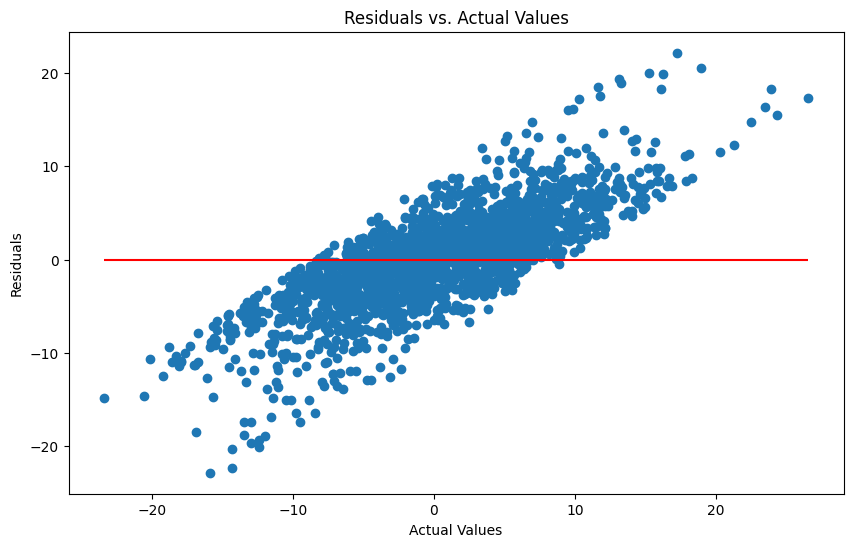
\includegraphics[width=\linewidth]{/Users/davidhunt/repos/learning/interview_problem_sets/Aquatic/data/residuals_first_model.png}  % Include the image
\end{figure}
\begin{figure}[h!]  % The figure environment
    \centering  % Center the image
    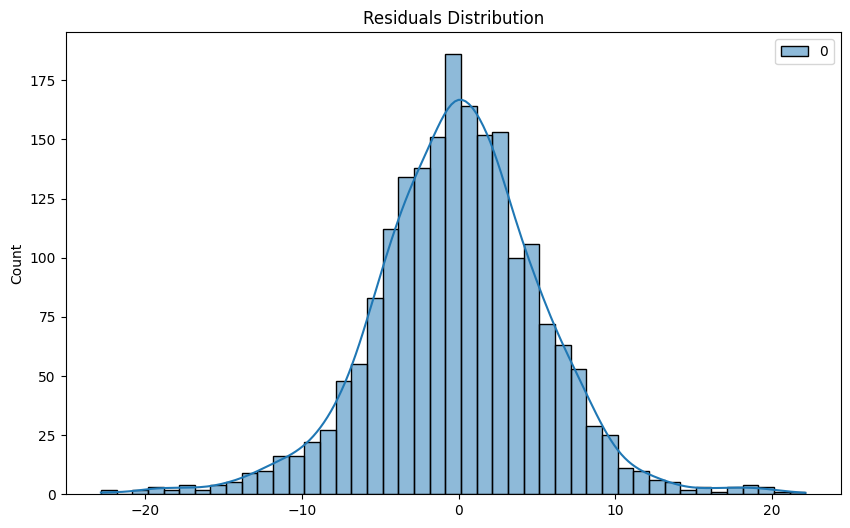
\includegraphics[width=\linewidth]{/Users/davidhunt/repos/learning/interview_problem_sets/Aquatic/data/residuals_dist_first_model.png}  % Include the image
\end{figure}
\pagebreak
\subsection*{Part 3}
Adding the features from Z greatly improved the quality of the model.
\begin{itemize}
    \item MSE of model: 20.86
    \item RMSE of model: 4.57
    \item R² of model: 0.55
    \item MAPE of model: 2.21
    \item Cross-Validated MSE: 21.81 ± 0.73
\end{itemize}

This suggests that ~55\% of the variance in the data is explained by the model and that the predictions are off by ~2\% on average still.
There still seems to be some linear relationship in the residuals though. 
\begin{figure}[h!]  % The figure environment
    \centering  % Center the image
    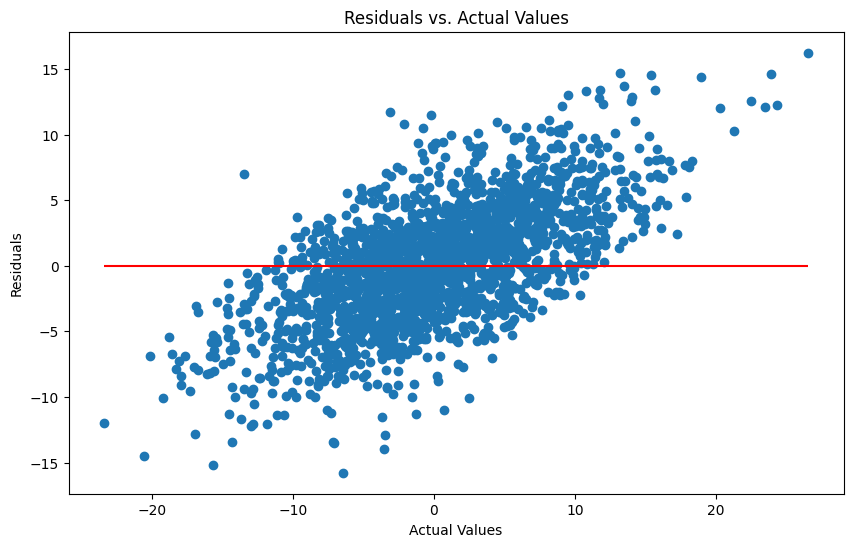
\includegraphics[width=\linewidth]{/Users/davidhunt/repos/learning/interview_problem_sets/Aquatic/data/residuals_second_model.png }  % Include the image
\end{figure}

\subsection*{Part 4}
The model is still not perfect but it is much better than the first model when including the additional features from Z.
The residuals are still normally distributed and the overall predictive \textit{miss} is still low at ~2\%.
However there is still clearly some linear relationship in the residuals that I'm missing as ideally this would be a random scatterplot
Overall the second model has higher predictive power with less error, but If I had more time I would like to train some additional higher power models to see if I could get a better fit.

\subsection*{Sources of Error}
\begin{itemize}
    \item I feel like there could be a scaling error in the features that I did not account for. I tried using a standard scalar but it did not improve the model much. 
    \item In addition, the winsorization I did could have removed some informative outliers, rather than bad ones, that could have improved the model.
    \end{itemize}
\end{document}